% Generated by ArticleSignalDiagrams. Opaque vector fills only.
\documentclass[10pt,tikz,border=5pt]{standalone}
\usepackage{lmodern}
\usetikzlibrary{fit}
\begin{document}
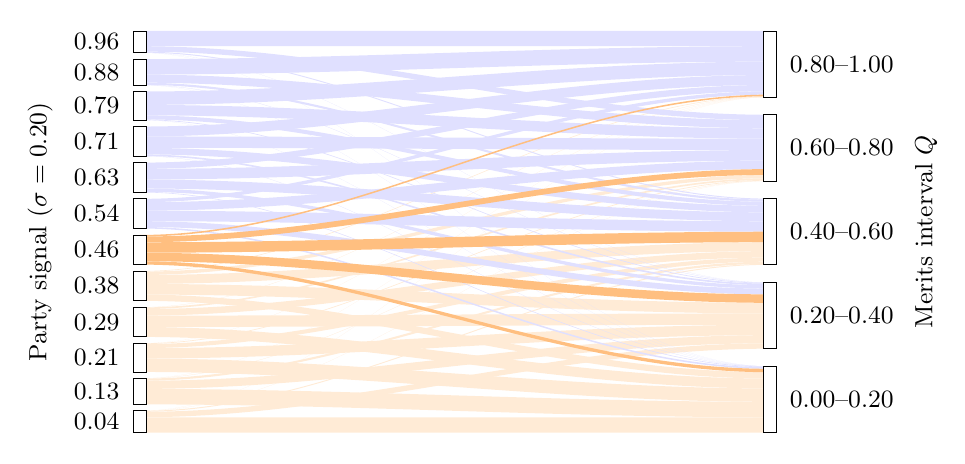
\begin{tikzpicture}[x=1cm,y=1cm,font=\small]\path[fill=orange!16!white,draw=none] (3.3,-5.1) .. controls (6,-5.1) and (8.6,-5.1) .. (11.3,-5.1) -- (11.3,-4.906438) .. controls (8.6,-4.906438) and (6,-4.906438) .. (3.3,-4.906438) -- cycle;
\path[fill=orange!16!white,draw=none] (3.3,-4.906438) .. controls (6,-4.906438) and (8.6,-4.035) .. (11.3,-4.035) -- (11.3,-3.966399) .. controls (8.6,-3.966399) and (6,-4.837838) .. (3.3,-4.837838) -- cycle;
\path[fill=orange!16!white,draw=none] (3.3,-4.837838) .. controls (6,-4.837838) and (8.6,-2.97) .. (11.3,-2.97) -- (11.3,-2.957597) .. controls (8.6,-2.957597) and (6,-4.825435) .. (3.3,-4.825435) -- cycle;
\path[fill=orange!16!white,draw=none] (3.3,-4.825435) .. controls (6,-4.825435) and (8.6,-1.905) .. (11.3,-1.905) -- (11.3,-1.904006) .. controls (8.6,-1.904006) and (6,-4.824441) .. (3.3,-4.824441) -- cycle;
\path[fill=orange!16!white,draw=none] (3.3,-4.824441) .. controls (6,-4.824441) and (8.6,-0.84) .. (11.3,-0.84) -- (11.3,-0.839963) .. controls (8.6,-0.839963) and (6,-4.824403) .. (3.3,-4.824403) -- cycle;
\path[fill=orange!16!white,draw=none] (3.3,-4.742585) .. controls (6,-4.742585) and (8.6,-4.906438) .. (11.3,-4.906438) -- (11.3,-4.710107) .. controls (8.6,-4.710107) and (6,-4.546254) .. (3.3,-4.546254) -- cycle;
\path[fill=orange!16!white,draw=none] (3.3,-4.546254) .. controls (6,-4.546254) and (8.6,-3.966399) .. (11.3,-3.966399) -- (11.3,-3.863504) .. controls (8.6,-3.863504) and (6,-4.443359) .. (3.3,-4.443359) -- cycle;
\path[fill=orange!16!white,draw=none] (3.3,-4.443359) .. controls (6,-4.443359) and (8.6,-2.957597) .. (11.3,-2.957597) -- (11.3,-2.930224) .. controls (8.6,-2.930224) and (6,-4.415986) .. (3.3,-4.415986) -- cycle;
\path[fill=orange!16!white,draw=none] (3.3,-4.415986) .. controls (6,-4.415986) and (8.6,-1.904006) .. (11.3,-1.904006) -- (11.3,-1.900768) .. controls (8.6,-1.900768) and (6,-4.412748) .. (3.3,-4.412748) -- cycle;
\path[fill=orange!16!white,draw=none] (3.3,-4.412748) .. controls (6,-4.412748) and (8.6,-0.839963) .. (11.3,-0.839963) -- (11.3,-0.839781) .. controls (8.6,-0.839781) and (6,-4.412566) .. (3.3,-4.412566) -- cycle;
\path[fill=orange!16!white,draw=none] (3.3,-4.330748) .. controls (6,-4.330748) and (8.6,-4.710107) .. (11.3,-4.710107) -- (11.3,-4.539969) .. controls (8.6,-4.539969) and (6,-4.16061) .. (3.3,-4.16061) -- cycle;
\path[fill=orange!16!white,draw=none] (3.3,-4.16061) .. controls (6,-4.16061) and (8.6,-3.863504) .. (11.3,-3.863504) -- (11.3,-3.731736) .. controls (8.6,-3.731736) and (6,-4.028842) .. (3.3,-4.028842) -- cycle;
\path[fill=orange!16!white,draw=none] (3.3,-4.028842) .. controls (6,-4.028842) and (8.6,-2.930224) .. (11.3,-2.930224) -- (11.3,-2.878716) .. controls (8.6,-2.878716) and (6,-3.977334) .. (3.3,-3.977334) -- cycle;
\path[fill=orange!16!white,draw=none] (3.3,-3.977334) .. controls (6,-3.977334) and (8.6,-1.900768) .. (11.3,-1.900768) -- (11.3,-1.891792) .. controls (8.6,-1.891792) and (6,-3.968359) .. (3.3,-3.968359) -- cycle;
\path[fill=orange!16!white,draw=none] (3.3,-3.968359) .. controls (6,-3.968359) and (8.6,-0.839781) .. (11.3,-0.839781) -- (11.3,-0.839034) .. controls (8.6,-0.839034) and (6,-3.967611) .. (3.3,-3.967611) -- cycle;
\path[fill=orange!16!white,draw=none] (3.3,-3.885793) .. controls (6,-3.885793) and (8.6,-4.539969) .. (11.3,-4.539969) -- (11.3,-4.413991) .. controls (8.6,-4.413991) and (6,-3.759815) .. (3.3,-3.759815) -- cycle;
\path[fill=orange!16!white,draw=none] (3.3,-3.759815) .. controls (6,-3.759815) and (8.6,-3.731736) .. (11.3,-3.731736) -- (11.3,-3.587606) .. controls (8.6,-3.587606) and (6,-3.615685) .. (3.3,-3.615685) -- cycle;
\path[fill=orange!16!white,draw=none] (3.3,-3.615685) .. controls (6,-3.615685) and (8.6,-2.878716) .. (11.3,-2.878716) -- (11.3,-2.796021) .. controls (8.6,-2.796021) and (6,-3.53299) .. (3.3,-3.53299) -- cycle;
\path[fill=orange!16!white,draw=none] (3.3,-3.53299) .. controls (6,-3.53299) and (8.6,-1.891792) .. (11.3,-1.891792) -- (11.3,-1.870595) .. controls (8.6,-1.870595) and (6,-3.511793) .. (3.3,-3.511793) -- cycle;
\path[fill=orange!16!white,draw=none] (3.3,-3.511793) .. controls (6,-3.511793) and (8.6,-0.839034) .. (11.3,-0.839034) -- (11.3,-0.836416) .. controls (8.6,-0.836416) and (6,-3.509175) .. (3.3,-3.509175) -- cycle;
\path[fill=orange!16!white,draw=none] (3.3,-3.427357) .. controls (6,-3.427357) and (8.6,-4.413991) .. (11.3,-4.413991) -- (11.3,-4.334299) .. controls (8.6,-4.334299) and (6,-3.347665) .. (3.3,-3.347665) -- cycle;
\path[fill=orange!16!white,draw=none] (3.3,-3.347665) .. controls (6,-3.347665) and (8.6,-3.587606) .. (11.3,-3.587606) -- (11.3,-3.45292) .. controls (8.6,-3.45292) and (6,-3.21298) .. (3.3,-3.21298) -- cycle;
\path[fill=orange!16!white,draw=none] (3.3,-3.21298) .. controls (6,-3.21298) and (8.6,-2.796021) .. (11.3,-2.796021) -- (11.3,-2.682679) .. controls (8.6,-2.682679) and (6,-3.099637) .. (3.3,-3.099637) -- cycle;
\path[fill=orange!16!white,draw=none] (3.3,-3.099637) .. controls (6,-3.099637) and (8.6,-1.870595) .. (11.3,-1.870595) -- (11.3,-1.827917) .. controls (8.6,-1.827917) and (6,-3.056959) .. (3.3,-3.056959) -- cycle;
\path[fill=orange!16!white,draw=none] (3.3,-3.056959) .. controls (6,-3.056959) and (8.6,-0.836416) .. (11.3,-0.836416) -- (11.3,-0.828607) .. controls (8.6,-0.828607) and (6,-3.04915) .. (3.3,-3.04915) -- cycle;
\path[fill=blue!12!white,draw=none] (3.3,-2.509091) .. controls (6,-2.509091) and (8.6,-4.291246) .. (11.3,-4.291246) -- (11.3,-4.271393) .. controls (8.6,-4.271393) and (6,-2.489238) .. (3.3,-2.489238) -- cycle;
\path[fill=blue!12!white,draw=none] (3.3,-2.489238) .. controls (6,-2.489238) and (8.6,-3.345397) .. (11.3,-3.345397) -- (11.3,-3.272083) .. controls (8.6,-3.272083) and (6,-2.415923) .. (3.3,-2.415923) -- cycle;
\path[fill=blue!12!white,draw=none] (3.3,-2.415923) .. controls (6,-2.415923) and (8.6,-2.55) .. (11.3,-2.55) -- (11.3,-2.417321) .. controls (8.6,-2.417321) and (6,-2.283244) .. (3.3,-2.283244) -- cycle;
\path[fill=blue!12!white,draw=none] (3.3,-2.283244) .. controls (6,-2.283244) and (8.6,-1.754603) .. (11.3,-1.754603) -- (11.3,-1.64708) .. controls (8.6,-1.64708) and (6,-2.175721) .. (3.3,-2.175721) -- cycle;
\path[fill=blue!12!white,draw=none] (3.3,-2.175721) .. controls (6,-2.175721) and (8.6,-0.808754) .. (11.3,-0.808754) -- (11.3,-0.765701) .. controls (8.6,-0.765701) and (6,-2.132668) .. (3.3,-2.132668) -- cycle;
\path[fill=blue!12!white,draw=none] (3.3,-2.05085) .. controls (6,-2.05085) and (8.6,-4.271393) .. (11.3,-4.271393) -- (11.3,-4.263584) .. controls (8.6,-4.263584) and (6,-2.043041) .. (3.3,-2.043041) -- cycle;
\path[fill=blue!12!white,draw=none] (3.3,-2.043041) .. controls (6,-2.043041) and (8.6,-3.272083) .. (11.3,-3.272083) -- (11.3,-3.229405) .. controls (8.6,-3.229405) and (6,-2.000363) .. (3.3,-2.000363) -- cycle;
\path[fill=blue!12!white,draw=none] (3.3,-2.000363) .. controls (6,-2.000363) and (8.6,-2.417321) .. (11.3,-2.417321) -- (11.3,-2.303979) .. controls (8.6,-2.303979) and (6,-1.88702) .. (3.3,-1.88702) -- cycle;
\path[fill=blue!12!white,draw=none] (3.3,-1.88702) .. controls (6,-1.88702) and (8.6,-1.64708) .. (11.3,-1.64708) -- (11.3,-1.512394) .. controls (8.6,-1.512394) and (6,-1.752335) .. (3.3,-1.752335) -- cycle;
\path[fill=blue!12!white,draw=none] (3.3,-1.752335) .. controls (6,-1.752335) and (8.6,-0.765701) .. (11.3,-0.765701) -- (11.3,-0.686009) .. controls (8.6,-0.686009) and (6,-1.672643) .. (3.3,-1.672643) -- cycle;
\path[fill=blue!12!white,draw=none] (3.3,-1.590825) .. controls (6,-1.590825) and (8.6,-4.263584) .. (11.3,-4.263584) -- (11.3,-4.260966) .. controls (8.6,-4.260966) and (6,-1.588207) .. (3.3,-1.588207) -- cycle;
\path[fill=blue!12!white,draw=none] (3.3,-1.588207) .. controls (6,-1.588207) and (8.6,-3.229405) .. (11.3,-3.229405) -- (11.3,-3.208208) .. controls (8.6,-3.208208) and (6,-1.56701) .. (3.3,-1.56701) -- cycle;
\path[fill=blue!12!white,draw=none] (3.3,-1.56701) .. controls (6,-1.56701) and (8.6,-2.303979) .. (11.3,-2.303979) -- (11.3,-2.221284) .. controls (8.6,-2.221284) and (6,-1.484315) .. (3.3,-1.484315) -- cycle;
\path[fill=blue!12!white,draw=none] (3.3,-1.484315) .. controls (6,-1.484315) and (8.6,-1.512394) .. (11.3,-1.512394) -- (11.3,-1.368264) .. controls (8.6,-1.368264) and (6,-1.340185) .. (3.3,-1.340185) -- cycle;
\path[fill=blue!12!white,draw=none] (3.3,-1.340185) .. controls (6,-1.340185) and (8.6,-0.686009) .. (11.3,-0.686009) -- (11.3,-0.560031) .. controls (8.6,-0.560031) and (6,-1.214207) .. (3.3,-1.214207) -- cycle;
\path[fill=blue!12!white,draw=none] (3.3,-1.132389) .. controls (6,-1.132389) and (8.6,-4.260966) .. (11.3,-4.260966) -- (11.3,-4.260219) .. controls (8.6,-4.260219) and (6,-1.131641) .. (3.3,-1.131641) -- cycle;
\path[fill=blue!12!white,draw=none] (3.3,-1.131641) .. controls (6,-1.131641) and (8.6,-3.208208) .. (11.3,-3.208208) -- (11.3,-3.199232) .. controls (8.6,-3.199232) and (6,-1.122666) .. (3.3,-1.122666) -- cycle;
\path[fill=blue!12!white,draw=none] (3.3,-1.122666) .. controls (6,-1.122666) and (8.6,-2.221284) .. (11.3,-2.221284) -- (11.3,-2.169776) .. controls (8.6,-2.169776) and (6,-1.071158) .. (3.3,-1.071158) -- cycle;
\path[fill=blue!12!white,draw=none] (3.3,-1.071158) .. controls (6,-1.071158) and (8.6,-1.368264) .. (11.3,-1.368264) -- (11.3,-1.236496) .. controls (8.6,-1.236496) and (6,-0.93939) .. (3.3,-0.93939) -- cycle;
\path[fill=blue!12!white,draw=none] (3.3,-0.93939) .. controls (6,-0.93939) and (8.6,-0.560031) .. (11.3,-0.560031) -- (11.3,-0.389893) .. controls (8.6,-0.389893) and (6,-0.769252) .. (3.3,-0.769252) -- cycle;
\path[fill=blue!12!white,draw=none] (3.3,-0.687434) .. controls (6,-0.687434) and (8.6,-4.260219) .. (11.3,-4.260219) -- (11.3,-4.260037) .. controls (8.6,-4.260037) and (6,-0.687252) .. (3.3,-0.687252) -- cycle;
\path[fill=blue!12!white,draw=none] (3.3,-0.687252) .. controls (6,-0.687252) and (8.6,-3.199232) .. (11.3,-3.199232) -- (11.3,-3.195994) .. controls (8.6,-3.195994) and (6,-0.684014) .. (3.3,-0.684014) -- cycle;
\path[fill=blue!12!white,draw=none] (3.3,-0.684014) .. controls (6,-0.684014) and (8.6,-2.169776) .. (11.3,-2.169776) -- (11.3,-2.142403) .. controls (8.6,-2.142403) and (6,-0.656641) .. (3.3,-0.656641) -- cycle;
\path[fill=blue!12!white,draw=none] (3.3,-0.656641) .. controls (6,-0.656641) and (8.6,-1.236496) .. (11.3,-1.236496) -- (11.3,-1.133601) .. controls (8.6,-1.133601) and (6,-0.553746) .. (3.3,-0.553746) -- cycle;
\path[fill=blue!12!white,draw=none] (3.3,-0.553746) .. controls (6,-0.553746) and (8.6,-0.389893) .. (11.3,-0.389893) -- (11.3,-0.193562) .. controls (8.6,-0.193562) and (6,-0.357415) .. (3.3,-0.357415) -- cycle;
\path[fill=blue!12!white,draw=none] (3.3,-0.275597) .. controls (6,-0.275597) and (8.6,-4.260037) .. (11.3,-4.260037) -- (11.3,-4.26) .. controls (8.6,-4.26) and (6,-0.275559) .. (3.3,-0.275559) -- cycle;
\path[fill=blue!12!white,draw=none] (3.3,-0.275559) .. controls (6,-0.275559) and (8.6,-3.195994) .. (11.3,-3.195994) -- (11.3,-3.195) .. controls (8.6,-3.195) and (6,-0.274565) .. (3.3,-0.274565) -- cycle;
\path[fill=blue!12!white,draw=none] (3.3,-0.274565) .. controls (6,-0.274565) and (8.6,-2.142403) .. (11.3,-2.142403) -- (11.3,-2.13) .. controls (8.6,-2.13) and (6,-0.262162) .. (3.3,-0.262162) -- cycle;
\path[fill=blue!12!white,draw=none] (3.3,-0.262162) .. controls (6,-0.262162) and (8.6,-1.133601) .. (11.3,-1.133601) -- (11.3,-1.065) .. controls (8.6,-1.065) and (6,-0.193562) .. (3.3,-0.193562) -- cycle;
\path[fill=blue!12!white,draw=none] (3.3,-0.193562) .. controls (6,-0.193562) and (8.6,-0.193562) .. (11.3,-0.193562) -- (11.3,0) .. controls (8.6,0) and (6,0) .. (3.3,0) -- cycle;
\path[fill=orange!50!white,draw=none] (3.3,-2.967332) .. controls (6,-2.967332) and (8.6,-4.334299) .. (11.3,-4.334299) -- (11.3,-4.291246) .. controls (8.6,-4.291246) and (6,-2.924279) .. (3.3,-2.924279) -- cycle;
\path[fill=orange!50!white,draw=none] (3.3,-2.924279) .. controls (6,-2.924279) and (8.6,-3.45292) .. (11.3,-3.45292) -- (11.3,-3.345397) .. controls (8.6,-3.345397) and (6,-2.816756) .. (3.3,-2.816756) -- cycle;
\path[fill=orange!50!white,draw=none] (3.3,-2.816756) .. controls (6,-2.816756) and (8.6,-2.682679) .. (11.3,-2.682679) -- (11.3,-2.55) .. controls (8.6,-2.55) and (6,-2.684077) .. (3.3,-2.684077) -- cycle;
\path[fill=orange!50!white,draw=none] (3.3,-2.684077) .. controls (6,-2.684077) and (8.6,-1.827917) .. (11.3,-1.827917) -- (11.3,-1.754603) .. controls (8.6,-1.754603) and (6,-2.610762) .. (3.3,-2.610762) -- cycle;
\path[fill=orange!50!white,draw=none] (3.3,-2.610762) .. controls (6,-2.610762) and (8.6,-0.828607) .. (11.3,-0.828607) -- (11.3,-0.808754) .. controls (8.6,-0.808754) and (6,-2.590909) .. (3.3,-2.590909) -- cycle;
\coordinate (axis-midline-0) at (0,-2.55);
\path[fill=white,draw=black,line width=0.3pt] (3.22,-5.1) rectangle (3.38,-4.824403);
\node[anchor=east,fill=white,inner sep=2pt] (bucket-0-0-0) at (3.12,-4.962202) {0.04};
\path[fill=white,draw=black,line width=0.3pt] (3.22,-4.742585) rectangle (3.38,-4.412566);
\node[anchor=east,fill=white,inner sep=2pt] (bucket-0-0-1) at (3.12,-4.577576) {0.13};
\path[fill=white,draw=black,line width=0.3pt] (3.22,-4.330748) rectangle (3.38,-3.967611);
\node[anchor=east,fill=white,inner sep=2pt] (bucket-0-0-2) at (3.12,-4.14918) {0.21};
\path[fill=white,draw=black,line width=0.3pt] (3.22,-3.885793) rectangle (3.38,-3.509175);
\node[anchor=east,fill=white,inner sep=2pt] (bucket-0-0-3) at (3.12,-3.697484) {0.29};
\path[fill=white,draw=black,line width=0.3pt] (3.22,-3.427357) rectangle (3.38,-3.04915);
\node[anchor=east,fill=white,inner sep=2pt] (bucket-0-0-4) at (3.12,-3.238254) {0.38};
\path[fill=white,draw=black,line width=0.3pt] (3.22,-2.967332) rectangle (3.38,-2.590909);
\node[anchor=east,fill=white,inner sep=2pt] (bucket-0-0-5) at (3.12,-2.779121) {0.46};
\path[fill=white,draw=black,line width=0.3pt] (3.22,-2.509091) rectangle (3.38,-2.132668);
\node[anchor=east,fill=white,inner sep=2pt] (bucket-0-0-6) at (3.12,-2.320879) {0.54};
\path[fill=white,draw=black,line width=0.3pt] (3.22,-2.05085) rectangle (3.38,-1.672643);
\node[anchor=east,fill=white,inner sep=2pt] (bucket-0-0-7) at (3.12,-1.861746) {0.63};
\path[fill=white,draw=black,line width=0.3pt] (3.22,-1.590825) rectangle (3.38,-1.214207);
\node[anchor=east,fill=white,inner sep=2pt] (bucket-0-0-8) at (3.12,-1.402516) {0.71};
\path[fill=white,draw=black,line width=0.3pt] (3.22,-1.132389) rectangle (3.38,-0.769252);
\node[anchor=east,fill=white,inner sep=2pt] (bucket-0-0-9) at (3.12,-0.95082) {0.79};
\path[fill=white,draw=black,line width=0.3pt] (3.22,-0.687434) rectangle (3.38,-0.357415);
\node[anchor=east,fill=white,inner sep=2pt] (bucket-0-0-10) at (3.12,-0.522424) {0.88};
\path[fill=white,draw=black,line width=0.3pt] (3.22,-0.275597) rectangle (3.38,0);
\node[anchor=east,fill=white,inner sep=2pt] (bucket-0-0-11) at (3.12,-0.137798) {0.96};
\node[fit=(bucket-0-0-0) (bucket-0-0-1) (bucket-0-0-2) (bucket-0-0-3) (bucket-0-0-4) (bucket-0-0-5) (bucket-0-0-6) (bucket-0-0-7) (bucket-0-0-8) (bucket-0-0-9) (bucket-0-0-10) (bucket-0-0-11),inner sep=0pt] (source-labels-0) {};
\coordinate (axis-title-0-0) at (source-labels-0.west |- axis-midline-0);
\node[rotate=90,anchor=south,inner sep=0pt] at ([xshift=-0.18cm]axis-title-0-0) {Party signal ($\sigma=0.20$)};
\path[fill=white,draw=black,line width=0.3pt] (11.22,-5.1) rectangle (11.38,-4.26);
\node[anchor=west,fill=white,inner sep=2pt] (bucket-0-1-0) at (11.48,-4.68) {0.00--0.20};
\path[fill=white,draw=black,line width=0.3pt] (11.22,-4.035) rectangle (11.38,-3.195);
\node[anchor=west,fill=white,inner sep=2pt] (bucket-0-1-1) at (11.48,-3.615) {0.20--0.40};
\path[fill=white,draw=black,line width=0.3pt] (11.22,-2.97) rectangle (11.38,-2.13);
\node[anchor=west,fill=white,inner sep=2pt] (bucket-0-1-2) at (11.48,-2.55) {0.40--0.60};
\path[fill=white,draw=black,line width=0.3pt] (11.22,-1.905) rectangle (11.38,-1.065);
\node[anchor=west,fill=white,inner sep=2pt] (bucket-0-1-3) at (11.48,-1.485) {0.60--0.80};
\path[fill=white,draw=black,line width=0.3pt] (11.22,-0.84) rectangle (11.38,-0);
\node[anchor=west,fill=white,inner sep=2pt] (bucket-0-1-4) at (11.48,-0.42) {0.80--1.00};
\node[fit=(bucket-0-1-0) (bucket-0-1-1) (bucket-0-1-2) (bucket-0-1-3) (bucket-0-1-4),inner sep=0pt] (destination-labels-0) {};
\coordinate (axis-title-0-1) at (destination-labels-0.east |- axis-midline-0);
\node[rotate=90,anchor=north,inner sep=0pt] at ([xshift=0.18cm]axis-title-0-1) {Merits interval $Q$};
\end{tikzpicture}
\end{document}

